% --------------------------------------------------------------------------------------
%                   LATEX TEMPLATE FOR DISSERTATION (HONS)
% --------------------------------------------------------------------------------------
\documentclass[11pt]{book}

\usepackage{amsfonts, amsmath, amssymb}  
\usepackage{times}

%\usepackage[backref=page,pagebackref=true,linkcolor = blue,citecolor = red]{hyperref}
%\usepackage[backref=page]{backref}

\usepackage{graphicx}
\DeclareGraphicsExtensions{.pdf,.png,.jpg}

\setlength{\oddsidemargin}{1.5cm}
\setlength{\evensidemargin}{0cm}
\setlength{\topmargin}{1mm}
\setlength{\headheight}{1.36cm}
\setlength{\headsep}{1.00cm}
%\setlength{\textheight}{20.84cm}
\setlength{\textheight}{19cm}
\setlength{\textwidth}{14.5cm}
\setlength{\marginparsep}{1mm}
\setlength{\marginparwidth}{3cm}
\setlength{\footskip}{2.36cm}


\begin{document}
\pagestyle{empty}

%: ----------------------------------------------------------------------
%:                  TITLE PAGE: name, degree,..
% ----------------------------------------------------------------------

\begin{center}

\vspace{1cm}

%%% Type the thesis title below%%%%%%%%%%%%%%%%
{\Huge         High-Performance Hadoop Map/Reduce R Interface Enhancement}

\vspace{25mm} 


\includegraphics[width=3.5cm]{logo}

 \vspace{35mm}

%%%%%Type Your Name Below%%%%%%%%%%%%
{\Large       Noah Zhang}

	\vspace{1ex}

Department of Statistics

The University of Auckland

	\vspace{5ex}

 %%%%%Typing Your Supervisors Name Below%%%%%%%%%%%%
Supervisor:             Simon Urbanek

	\vspace{30mm}

A dissertation submitted in partial fulfillment of the requirements for the degree of BSc(Hons) in Statistics, The University of Auckland, 2020.

\end{center}

\newpage


%: --------------------------------------------------------------
%:                  FRONT MATTER:  abstract,..
% --------------------------------------------------------------
\chapter*{Abstract}       
\setcounter{page}{1}
\pagestyle{headings}
% \pagenumbering{roman}

\addcontentsline{toc}{chapter}{Abstract}


 Put your abstract  here.  The abstract should contain a brief summary of the aim, methodologies, 
finding and conclusions of the dissertation.  The abstract should normally be fewer than 350 words.


One of the most widely used parallel programming models today is MapReduce. MapReduce is easy both to learn and use, and is especially useful in analyzing large datasets. While it is not suitable for several classes of scientific computing operations that are better served by message-passing interface or OpenMP, such as numerical linear algebra or finite element and finite difference computations, MapReduce's utility in workflows frequently called “big data” has made it a mainstay in high performance computing. This chapter introduces the MapReduce programming model and the Hadoop open-source framework which supports it.

Big data is concern massive amount, complex, growing data set from multiple autonomous sources. It has to deal with large
and complex dataset that can be structured, semi-structured or unstructured and will typically not fit into memory to be processed.
MapReduce is a programming model for processing large datasets distributed on a large clusters.A rapid growth of data in recent time,
Industries and academia required an intelligent data analysis tool that would be helpful to satisfy the need to analysis a large amount of
data. MapReduce framework is basically designed to compute data demanding applications to support effective decision making. Since
its introduction, remarkable research efforts have been put to make it more familiar to the users subsequently utilized to support the
execution of enormous data intensive applications. This survey paper highlights and investigates various applications using recent
MapReduce models.





%: --------------------------------------------------------------
%:                  END:  abstract
% --------------------------------------------------------------


%: ----------------------- contents ------------------------
\setcounter{secnumdepth}{3} % organisational level that receives a numbers
\setcounter{tocdepth}{3}    % print table of contents for level 3
\tableofcontents            % print the table of contents
% levels are: 0 - chapter, 1 - section, 2 - subsection, 3 - subsection

%: --------------------------------------------------------------
%:                  MAIN DOCUMENT SECTION
% --------------------------------------------------------------
	
\chapter{Introduction}%    \chapter{}  = level 1, top level

A thesis should always have an introduction.  The purpose is to describe the general subject area, state the research problem of interest, outline the main results of the thesis, and put the results in context with the wider subject area and its applications.

The main body of the text must be divided into a logical scheme which  is followed consistently throughout the work.  
 It usually starts with an introduction chapter  and ends with  a conclusion chapter. See, for example, the table of contents on page 3. 

There is strict  35-page limit  for an applied mathematics dissertation,  including  the references  but excluding  appendices. 

\chapter{Concept of Big Data}

Big data concerns huge amounts, complex and diverse sets of information that is growing at ever-increasing rates. The size of the data suggest that we will need to deviate from the traditional processing methodologies and to adapt an inexpensive and efficient way through distributed/parallel computing.\\

Today, we can find upwards of 800 million webpages providing documentation on big data. Enthusiasts believe that Big Data is the next big thing after Cloud [1]. 

\section{Characteristics of Big Data}

The concept of big data is generally vague without a formal definition, however the general consensus is that there are specific attributes that define big data The four characteristics of big data are Volume, Velocity, Variety and Veracity [2]. 

\begin{center}
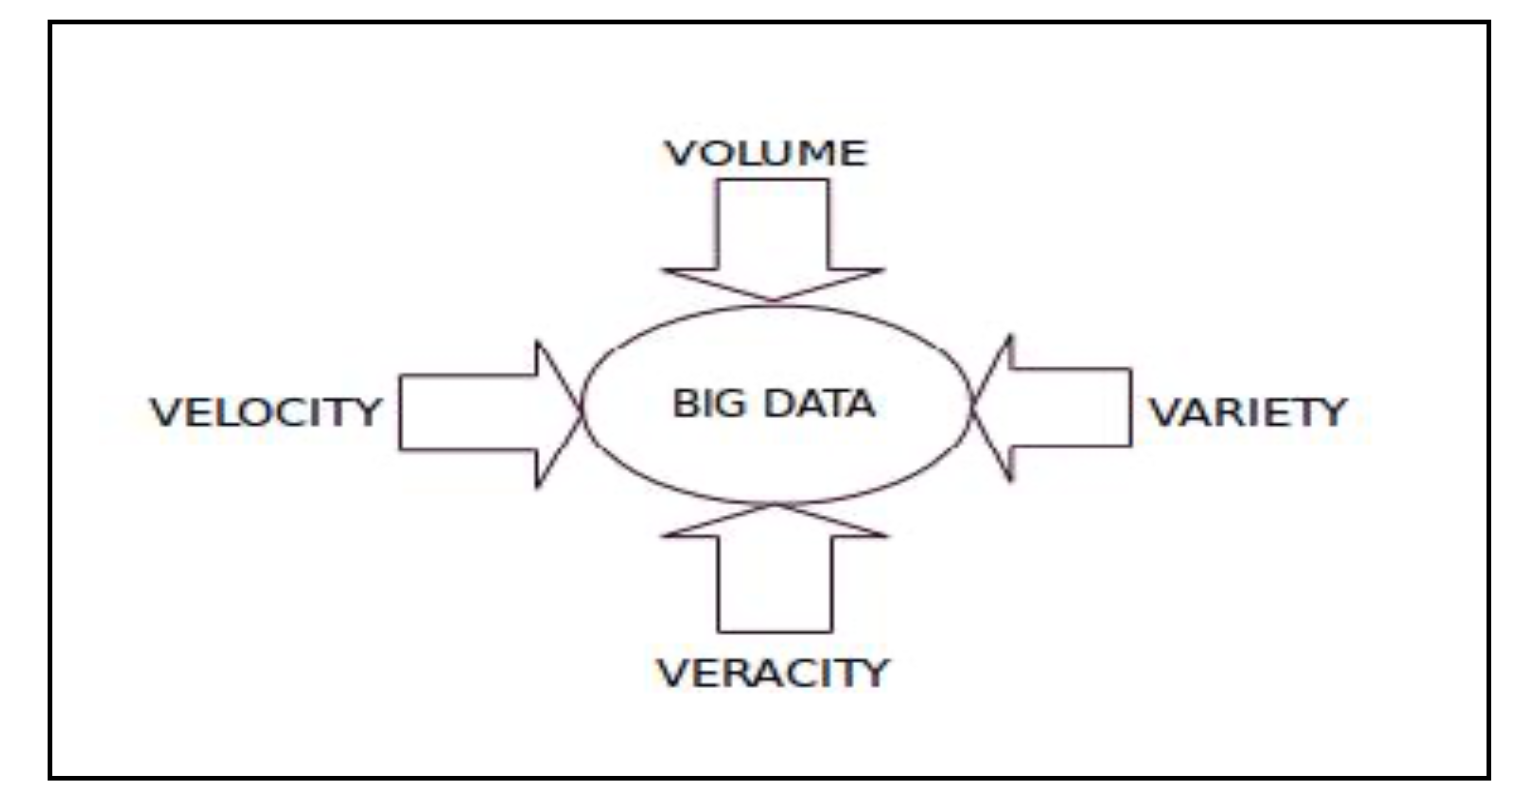
\includegraphics[width=10cm]{4vbd}\\
\end{center}

The main characteristic that makes data “big” is its sheer volume. According to estimates by IBM, we can expect at least 40 Zettabytes (43 Trillion Gigabytes) of data to be created in 2020 [3]. The volume of data sets being processed and analysed has reached sizes larger than terabytes and even petabytes. This suggests that data sets these days are becoming too large to process within a single desktop machine/processor. \\

Velocity is the speed at which data is generated. High velocity data is generated with such a pace that it may require certain distributed processing techniques. Good examples of high velocity data includes social media posts.\\

Variety is the source of the data which can be found in different forms such as text, numerical, images, audio and video records. The variety in the data will require distinct processing capabilities or algorithms to handle different formats. \\

Veracity is the quality of the data. Information may be volatile or incomplete seen in low veracity data sets containing a high percentage of meaningless data referred to as noise. On the other hand, high veracity data hold records that are valuable to analyse and contribute in a meaningful way to the overall results.

\section{Structure of Big Data} 

Big data can be categorised as structured or unstructured.\\
 
Structured data is usually stored and managed in relational databases with predefined data models. Examples of relational database applications with structured data include customer information, sales transactions, airline reservations systems, and billing systems. This type of structured data within relational databases can be accessed using Structured Query language (SQL).\\
 
Unstructured data, in contrast, has its internal structure but it is not structured through pre-defined data models or schema. As it may comes in many different formats, it cannot be stored in relational databases which also becomes a real challenge for systems to process and analyse. The unstructured data may be stored within non-relational databases like NoSQL.

\chapter{MapReduce Framework}

At present, with data being generated at an exponential rate, there is the need to deploy data intensive application and storage clusters in order to keep up with the amount of data. To handle such problem, Google developed the MapReduce programming model for distributed computing based on the Java language [5].

\section{Concept of MapReduce}

There are multiple approaches for processing relatively smaller datasets, however larger datasets require a different approach specifically for data that is too big to fit in memory. The traditional approach to process data on a single machine is to break data into individual chunks which is then loaded and processed sequentially on the machine. 

MapReduce is a processing technique/programming model for distributed computing based on Java. It is designed to process large datasets using the same splitting approach by breaking down the dataset into independent chunks. But instead of processing the chunks sequentially, the chunks are processed in parallel on a collective group of computers known as a cluster. The results of the individual chunks are then aggregated and returned as output.\\

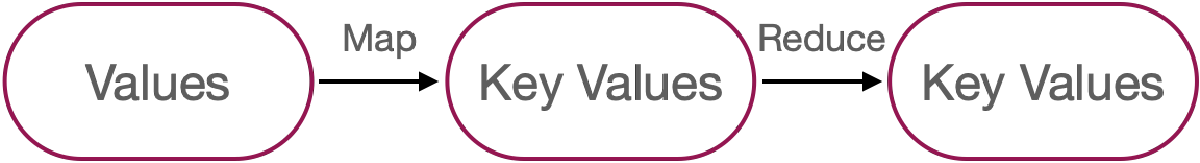
\includegraphics[width=8cm]{keyvalue} \\

The algorithm operates on key-value pairs, which means that it takes a set of input key-value pairs and produces a set of output key-value pairs. In addition, the user is required to specify two functions for the Mapper and Reducer. The Mapper takes the input and produce the intermediate key-value pairs which is passed to the Reducer to create a set of output key-value pairs. The Reducer combines all the values associated with each key to create a smaller set of values. This enables us to input data that may be too large to fit in standard memory.\\

In the simplest form of the MapReduce model, the user only specifies the Map function. In this case, the output will consist of the intermediate key-value pairs which is ordered by the keys. 

\section{The MapReduce Process}

The complete process typically consists of four operations namely, splitting, mapping, shuffling and reducing.\\

1. Splitting - the process will first break and divide the input data into fixed independent chunks which is passed to the map procedure. The default size of each chunk is 64MB, however this can be adjusted by the user. \\

2. Mapping - the purpose of the mapper is to process the input data. In this phase, data in each chunk is passed to a user specified map function and returns output in the form of key-value pairs. For example, if a file contains 100 lines to be processed, 100 mappers can run together to process one record each or if 50 mappers can run together to process two lines each. The Hadoop framework decides how many mappers to allocate based on the size of the data and the memory block available on each mapper server.\\

3. Shuffling - the process by which the intermediate output from the mappers is transferred to the reducer. The intermediate output is sorted automatically by key. key-value pairs which may contain 1 or more keys.

4. Reducing - In this phase, the output values from shuffling are aggregated. This should combine values from the intermediate values and return a single output value for each key. In other words, this operation is a summary of the complete dataset.

\section{Examples}



\section{Advantages of MapReduce}

The main advantage of MapReduce is that it is highly scalable. This is due to the ability to process large data sets across multiple computer nodes. These servers can be inexpensive and can also operate in parallel. This simple scalability is what attracts many to utilize the MapReduce model.

Other advantages include cost efficiency, security and authentication, parallel processing, availability, resilient and simple.


\chapter{The Hadoop Framework}

Hadoop is Apache's free and open-source implementation of the MapReduce framework. Apache Hadoop offers reliable, scalable, parallel and distributed computing scaling up from a single server to a network of multiple computers[4]. It was developed with the purpose of having a data store that allow organisations to leverage big data analytics with cost efficiency in mind.\\

%There are two main components of the Hadoop Framework: Storage and Processing

\section{Hadoop Architecture}

Hadoop follows a master/slave architecture design for data storage and distributed data processing using HDFS and MapReduce respectively. The master node for data storage is NameNode while the master node for parallel processing is the Job Tracker. The slave nodes are comprised of other machines in the Hadoop cluster which stores the data and performs the computations. Each slave node have a DataNode and a TaskTracker that synchronises the process respectively. \\

\begin{center}
 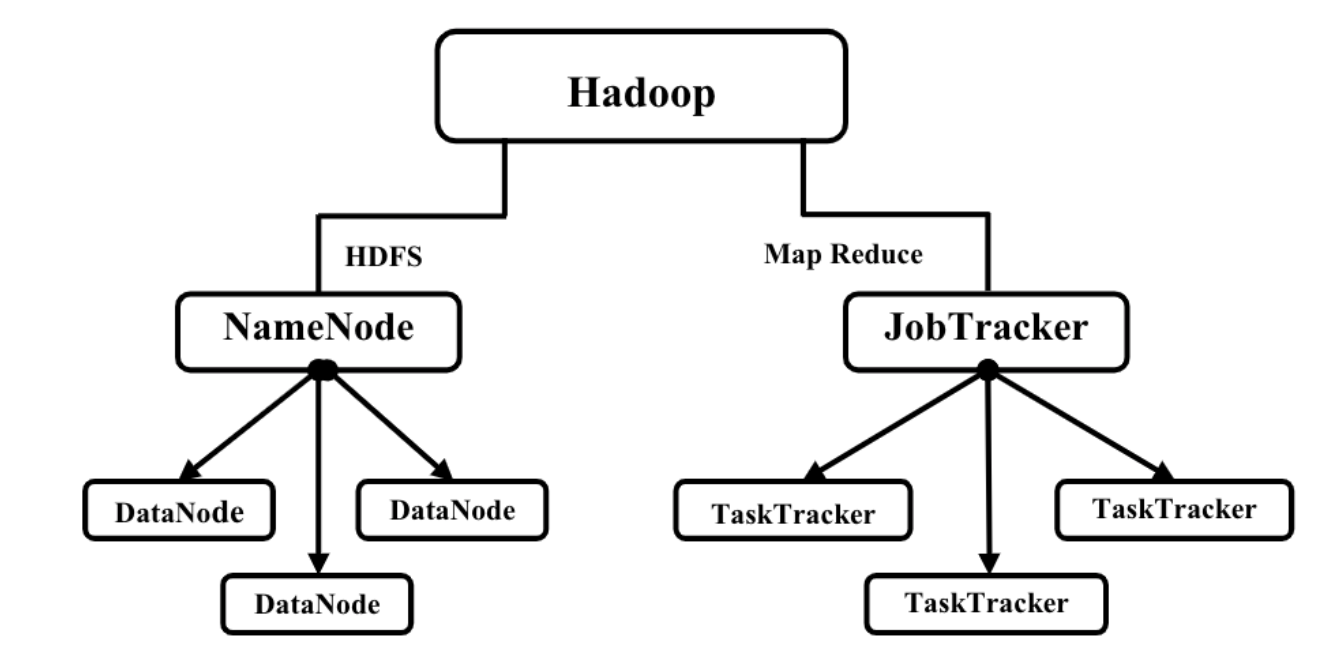
\includegraphics[width=10cm]{hadoop}\\
 \end{center}

The Hadoop system can be set up via cloud or locally. The cluster we will be running is a set up of 8 virtual machines.

\section{Storage - HDFS}

The storage component of the Hadoop architecture is known as the Hadoop Distributed File System (HDFS). The NameNode runs on the master node and manages metadata about the file system in a file named fsimage. This metadata is cached in main memory to provide faster access to the clients on read/write requests. The NameNode controls also manages the slaves by splitting files into chunks (default 64 megabytes) and distributing them across each DataNode in the cluster. The DataNodes are primary storage elements of HDFS where chunks of data are stored and replicated according to the instructions from the NameNode. Secondary NameNode is to periodically read the file system, log changes and applying them to the fsimage file. This will enable the NameNode to boot faster.\\

The main advantages of HDFS is data locality and fault tolerance. Data locality allow the nodes to manipulate the data they have access to which results in faster and more efficient processing while handling faults through the process of replicating files across each slave node[4].\\

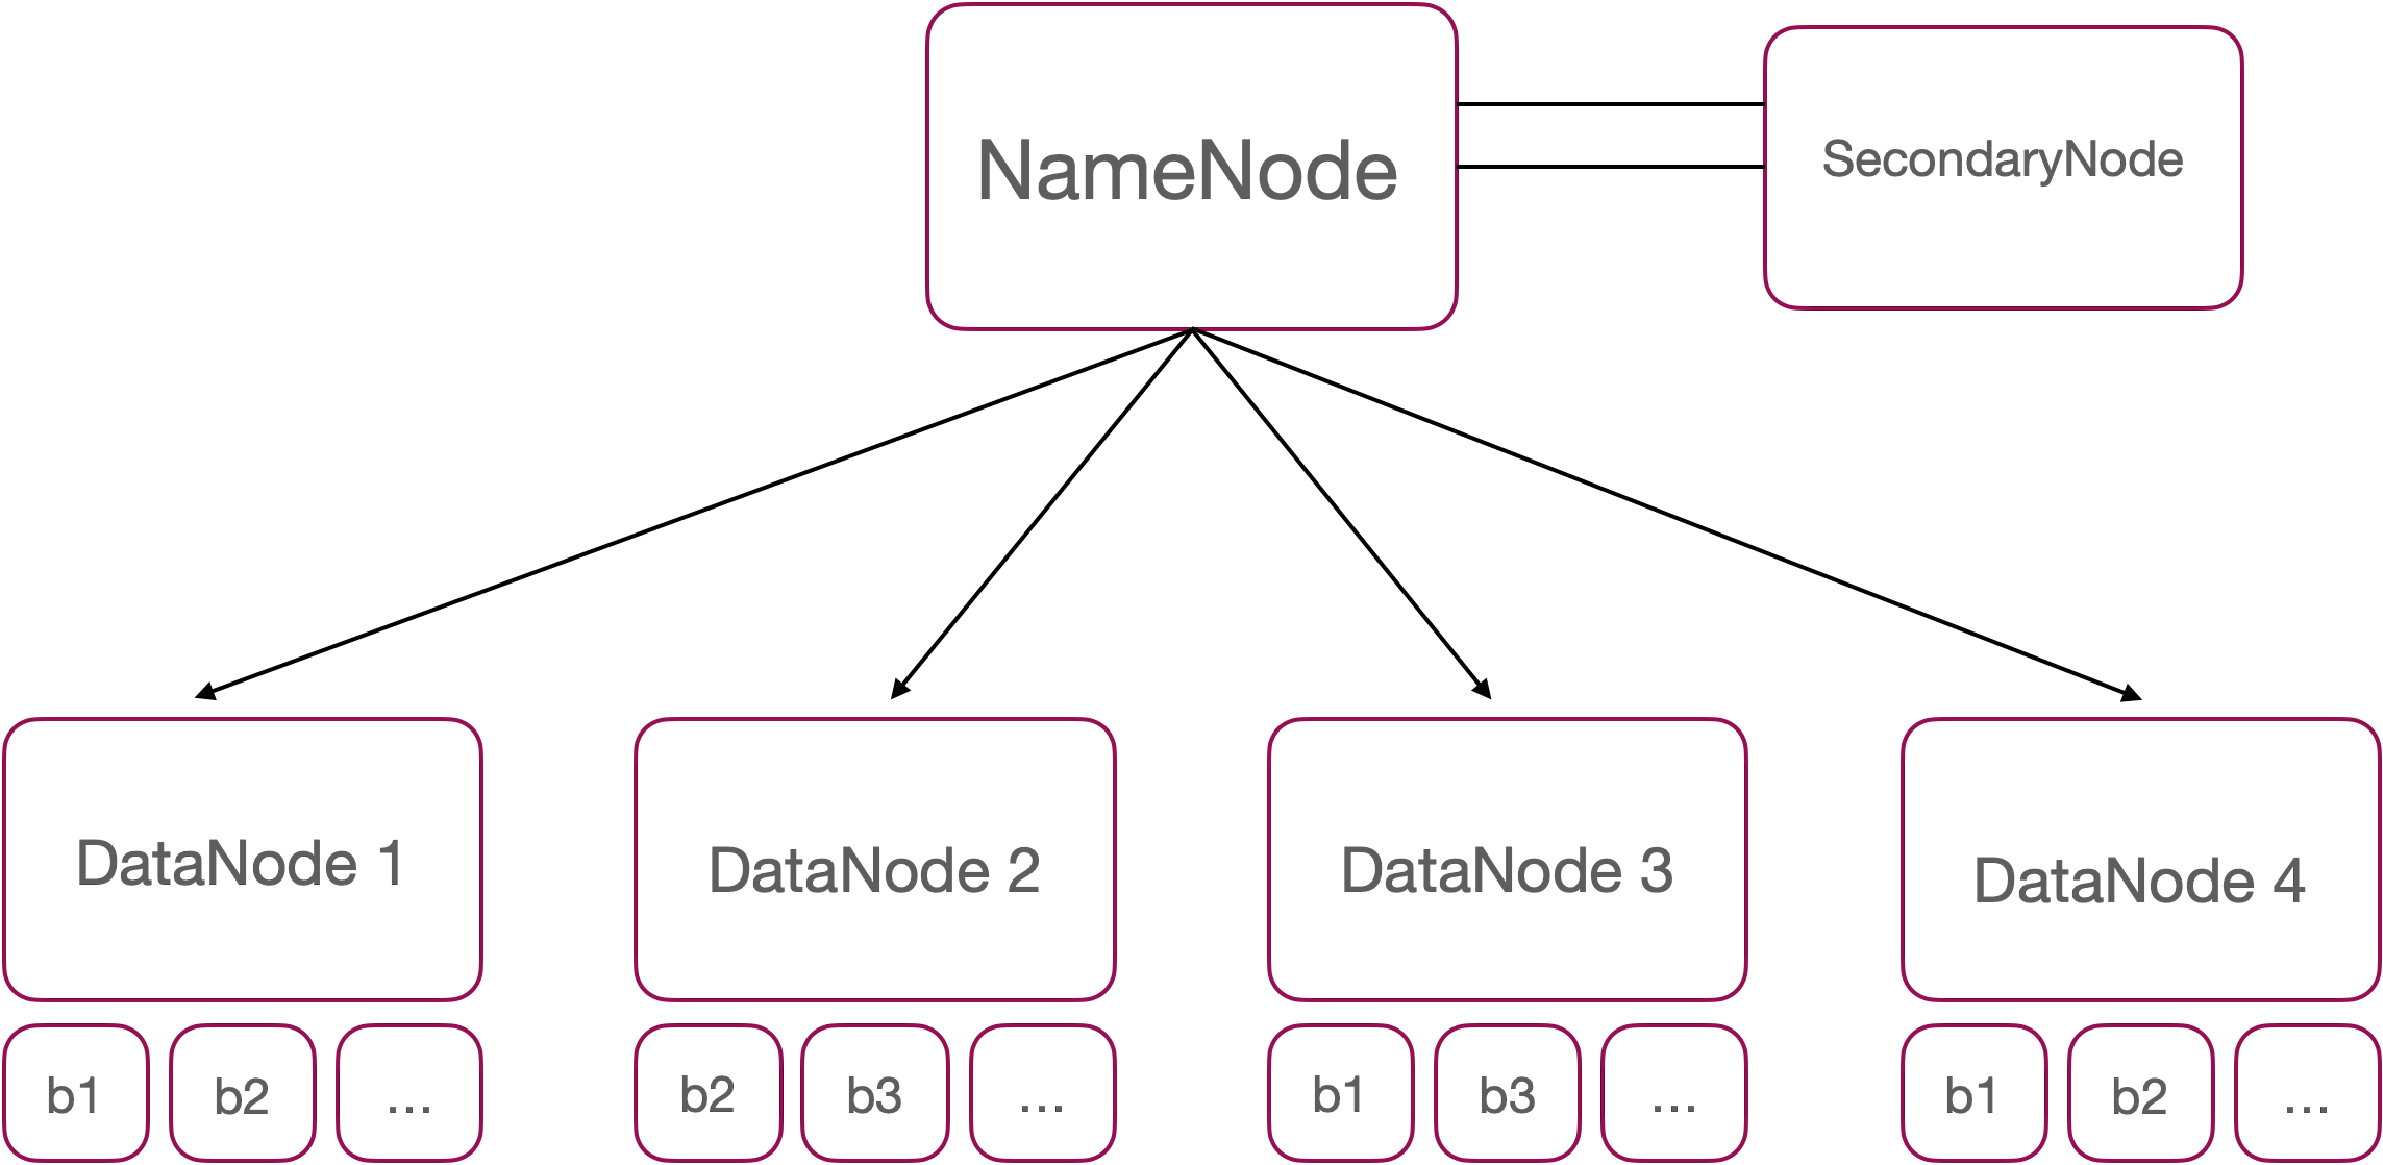
\includegraphics[width=8cm]{hdfs}

\section{Processing - MapReduce}

In a MapReduce job, the input is broken down into multiple chunks which are processed by the map phase and then the output of the map phase is passed as input to the reduce phase. The input and output files are stored in the file system, while the output of the map phase (known as intermediate results) are only stored temporarily in the process. As the process runs in parallel, the reduce task on specific nodes may begin once its map tasks is complete rather than waiting on all map tasks to complete.\\

Similar to HDFS, the MapReduce process also utilises the master/slave architecture in which the JobTracker runs on the master node while the TaskTracker runs on each slave node. \\

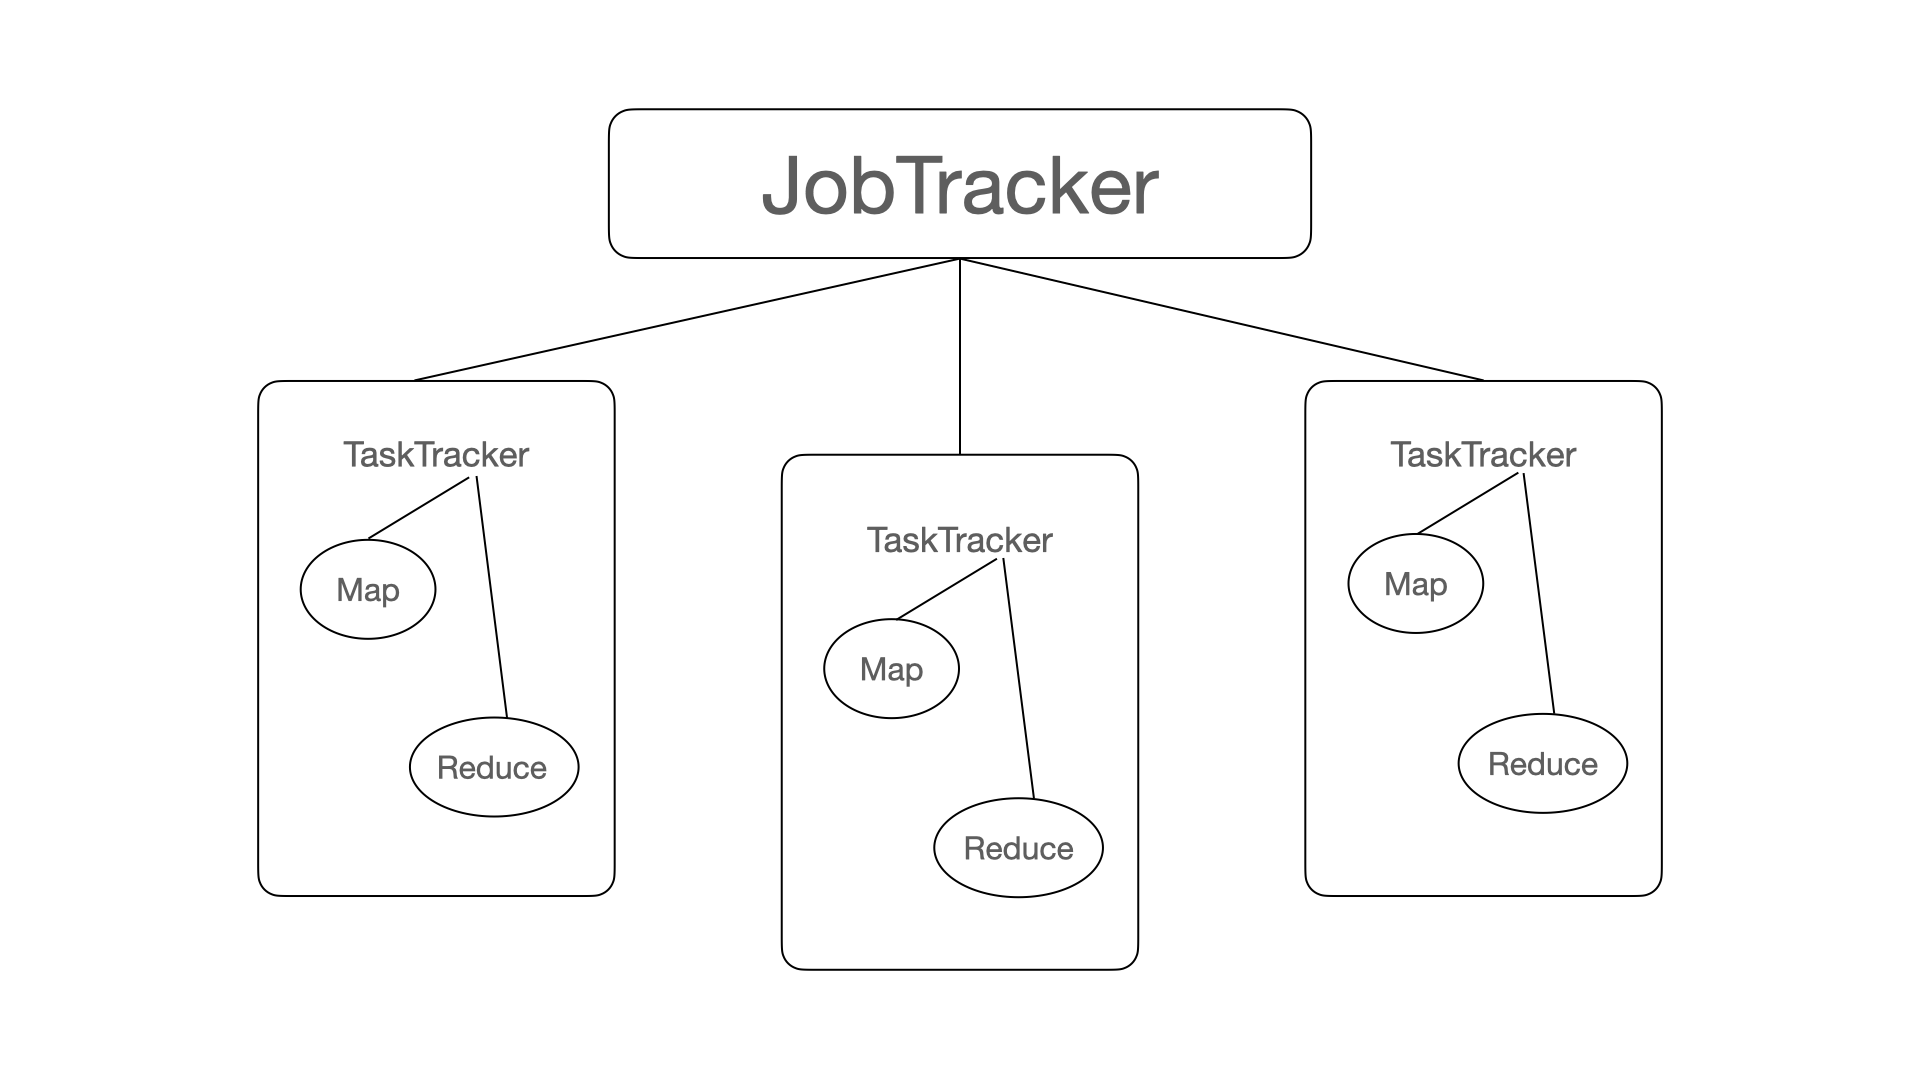
\includegraphics[width=8cm]{jobtracker}

The JobTracker monitors the MapReduce tasks carried out by the TaskTracker running on the slave nodes. The user will only interact with the master node by submitting jobs to the JobTracker. The JobTracker then locates and submits the jobs to the TaskTracker. The slave nodes are monitored by the JobTracker through heartbeat signals to determine whether a node has failed. The JobTracker is a point of failure for the Hadoop MapReduce service and if it goes down, all jobs will be stopped. \\

The TaskTracker runs on the slave nodes in a cluster and receives jobs from the JobTracker to execute the MapReduce tasks. Each TaskTracker has an allocation of task slots which indicate the number of tasks it can accept. The JobTracker will delegate jobs to the TaskTracker based on the number of available/empty slots while the TaskTracker will periodically send heartbeat signals to inform the JobTracker of any issues. TaskTracker failure is not considered fatal as tasks can be reallocated to another node when it becomes unresponsive.\\

\chapter{Hadoop Streaming}

Hadoop streaming is a utility that comes with the Hadoop distribution which allow users to create and run MapReduce jobs to be executed in the Hadoop cluster using other languages. By default the Hadoop MapReduce framework is written in Java but it utilizes Unix streams to pipe between Hadoop and our MapReduce program so we can use any language which can read standard input and write to standard output for our MapReduce program. MapReduce programs can be written in mutiple languages such as R, Python, Perl, PHP, C++, etc. The utility is packed in a JAR file. 

\section{Purpose}

Using the utility, we can create executable scripts to run MapReduce Jobs. Furthermore, we can create executable scripts to run the mapper and reducer functions which are passed to Hadoop streaming. The utility creates map and reduce jobs and submits them to the cluster which can then be monitored, thus enabling a person to write MapReduce job in the language of their choice without having any knowledge of Java.

\section{Syntax}

The syntax below can be used to run MapReduce jobs written in a different language to process data using the Hadoop MapReduce framework.\\

\begin{verbatim}
$HADOOP_HOME/bin/hadoop jar $HADOOP_HOME/hadoop-streaming.jar 
    -input myInputDirs 
    -output myOutputDir 
    -mapper /bin/cat 
    -reducer /usr/bin/wc
\end{verbatim}

The input command is used to provide the directory fo the input which the output command is used to provide the output directory. The mapper command is used to specify the executable mapper class while the reducer command is used to specify the executable reducer class.

The mapper command is used to specify the executable mapper class while the reducer command is used to specify the executable reducer class.

\section{How it Works}

Let us now explore how Hadoop streaming works.\\


\includegraphics[width=14cm]{streaming}\\

The mapper and reducer are scripts/functions created by the user that reads in the input line by line from standard input and returns the output to standard output. If the mapper script/function is specified, the mapper will converts the inputs into lines and converts the lines to the standard input which feeds into the mapper. In the process, the mapper converts each line into a key and value pair returned as standard output. If the reducer script/function is specified, the reducer then draws the line-oriented key value pairs from the mapper as standard input and converts each line collected into a key/value pair. This is then emitted to standard output. 

For both the mapper and the reducer, first entry of the line is the key followed by the value which is separate by a tab character. If there is no tab character in the line, then the entire line is considered as the key and the value is considered null. 

\section{Advantages}

1. Availability - the utility comes with the Hadoop distribution hence does not require further installation of softwares.\\
2. Learning - relatively easy to learn as it requires basic unix coding.\\
3. Reduce Development Time - it is much quicker to write mapper and reducer scripts/functions whereas using native Java MapReduce application is more complex as it requires the application to be complied, packaged, and exporting the JAR file.\\
4. Faster Conversion - it takes very little time to convert data from one format to another using Hadoop streaming especially when the input and output formats are specified.\\
5. Testing - input and output data can be tested quickly by using it with Unix or command line tools.

\chapter{HMR Hadoop MapReduce Package for R}

HMR is a package developed in R which acts as an interface which give R users the ability to execute Hadoop Map/Reduce jobs. It is highly efficient as it utilise chunk-wise processing as well as automated conversion to and from R objects. This allows users to feed existing R code to Hadoop with ease. There are other packages in R which uses the traditional key-value operations such as the rmr2 package.

\section{Functions in iotools}

HMR is highly efficient as it leverages the iotools package in R. It is a set of tools for quickly importing and processing datasets using any data source. The functions packaged in iotools are comparatively faster than the native functions in R as well as other packages such as bigmemory, readr, foreach, etc. 

The two functions chunk.reader and read.chunk are functions used in the HMR package. chunk.reader essentially converts a binary connection into chunks stored as an object in R while preserving the integrity of the lines. On the other hand, chunk.read converts this object into a raw vector for each subsequent chunk. The efficiency comes from the use of binary data and raw objects in R which allow fast chunk-wise processing. 

Other core functions in the iotools package used in the HMR package are mstrsplit and dstrsplit. It takes either a raw or character vector and splits it into a matrix or data frame in R with the specified separator. These functions are able to minimize the copying of data and avoid the use of intermediate strings to improve performance.


\section{Current Approach}

HMR can take two types of input objects: hpath and hinput. Hpath only contains the path of the input whereas hinput has an additional formatter argument which allows the user to specify the class of the input variables as a vector or a list. This will require the user to have some familiarity or knowledge of structure of the data. If no list or vector is specified for the formatter, then HMR defaults to the default formatter which uses the mstrsplit function with tab as the key separator and $\mid$ as the the column separator. With the default formatter, the class of the variables are in the string/character format which is highly inefficient. If separate formatters are required, the formatter can be a list with the entries map and/or reduce specifying the corresponding formatter function.

The problem with the default formatter is that it is highly inefficient to read in data as string/characters also it will require more coding in the map and reduce functions in order to read and process the data. 



\chapter{Package Enhancement - Automating Formatters}

The idea of this project is to make the HMR package more user-friendly while retaining efficiency. If we can automatically detect the format of the input data for both the map and reduce stage, then it makes it a lot easier to write the formatter functions. 

\section{New Approaches}

The enhancement provides automatic detection of the formatter for the mapper and the reducer instead of requiring the user to specify the formatters. The additional argument in the HMR function is autoformatter which is set to TRUE for dynamic detection, FALSE for static approach and defaults to NULL if the user wish to specify their own formatters in the function.

\subsection{Dynamic Approach}

The dynamic approach does the detection of the formatter during the MapReduce process. It is a function called coltypes which takes the split chunks in the form of raw vectors and returns a character vector containing the class of each attribute in the dataset. 

advantages: each chunk may vary, 
disadvantage: no header

\begin{verbatim}
  ## dynamic approach
  coltypes <- function(r, sep=formsep, nsep='\t', 
                       nrowsClasses=25L, chunksize=size, header=TRUE) {
    if (sum(r==10) < nrowsClasses) {
      nrowsClasses = sum(r==10)
      r <- r[1:chunksize]
      r <- r[1:tail(which(r==10),1)]
    }
    subset = mstrsplit(r, sep=sep, nsep=nsep, 
    			nrows=nrowsClasses, skip=header)
    colClasses = apply(subset, 2, function(x) 
    				class(type.convert(x, as.is=TRUE)))
    if (header) {
      col_names = mstrsplit(r, sep=sep, nsep=nsep, nrows=1)
      if ((length(col_names) - 1 == length(colClasses)) && !is.na(nsep))
        col_names = col_names[-1]
      names(colClasses) = col_names
    }
    colClasses
  }
\end{verbatim}

\subsection{Static Approach}

The static approach also detects the formatters but instead of running on each chunk of data, it reads an allocated chunk size starting from the top of the dataset. The chunk size can be specified by the user, however the default is set at 1 million bytes. Then it calls the same coltypes function on this allocated chunk of data to return the character vector containing the class of each attribute in the dataset.

The risk with this approach is data may be incomplete, i.e. may be logical due to missing values. More suitable for known structure.

\begin{verbatim}
  ## new static approach
  guess <- function(path, chunksize=size, header=TRUE, map) {
    f <- pipe(paste("hadoop fs -cat", shQuote(path)), "rb")
    cr <- chunk.reader(f)
    r <- read.chunk(cr, chunksize)
    colClasses = coltypes(r)
    close(f)
    if (!missing(map)) {
      m = map(dstrsplit(r, colClasses, sep=formsep, skip=header))
      c = coltypes(as.output(m), header=FALSE)
      if (length(c) == length(names(m)))
        names(c) = names(m)
      rm(list=c("cr", "r", "f"))
      list(map=function(x) dstrsplit(x, colClasses, 
      	sep=formsep, skip=header), 
           reduce=function(x) dstrsplit(x, c, sep="|", 
           	nsep="\t", skip=FALSE))
    }
    else function(x) dstrsplit(x, colClasses, sep=formsep, skip=header)
  }
  \end{verbatim}

\section{Formatter Logic}

\begin{verbatim}
  ## formatter logic
  map.formatter <- NULL
  red.formatter <- NULL
  if (!missing(formatter)) {
    if (is.list(formatter)) {
      map.formatter <- formatter$map
      red.formatter <- formatter$reduce
    } 
    else map.formatter <- red.formatter <- formatter
  }
  else {
    if (missing(autoformatter)) {
      if (inherits(input, "hinput"))
        map.formatter <- attr(input, "formatter")
      if (is.null(map.formatter)) map.formatter <- .default.formatter
      if (is.null(red.formatter)) red.formatter <- .default.formatter
    }
    else {
      if (isTRUE(autoformatter)) {
        map.formatter <- function(x) dstrsplit(x, coltypes(x), 
        	sep=formsep, skip=TRUE)
        if (!missing(reduce)) 
          red.formatter <- function(x) dstrsplit(x, 
          	coltypes(x, header=FALSE), nsep='\t')
      }
      else if (autoformatter==FALSE) {
        if (!missing(reduce)) {
          formatter <- guess(paste0(input,"/*"), map=map)
          map.formatter <- formatter$map
          red.formatter <- formatter$reduce
        }
        else map.formatter <- guess(paste0(input,"/*"))
      }
    }
  }
  \end{verbatim}



\section{Examples}







\subsection{Equations}
The main strength of LaTex is  mathematical typesetting.  

There is a huge amount of information about LaTex on the internet.
A helpful short manual, also included in this folder, is the file
\verb+latex_intro.pdf+
This document gives a lot of sample LaTex commands.  
The file \verb+latex-howto.tex+ in this folder also contains examples of many latex commands.




We first show  some simple examples of 
mathematical formulae using latex typesetting.





\chapter{References}
1. BIG DATA: Challenges and opportunities, Infosys Lab Briefings,
Vol 11 No 1, 2013. \\

2. Big Data And Hadoop: A Review Paper, Rahul Beakta, 2015 \\

 3. IBM Big Data analytics HUB,
www.ibmbigdatahub.com/infographic/four-vs-big-data

4. Hadoop, MapReduce and HDFS: A Developers Perspective, 
Mohd Rehan Ghazi, Durgaprasad Gangodkar, 2015

5. MapReduce: Simplified Data Processing on Large Clusters, 
Jeffrey Dean and Sanjay Ghemawat

6. iotools: High-Performance I/O Tools for R, 
Taylor Arnold, Michael J. Kane, and Simon Urbanek


\end{document}
